% !TEX encoding = UTF-8 Unicode

\documentclass[a4paper]{article}

\usepackage[utf8x,utf8]{inputenc}
\usepackage[T1]{fontenc}
\usepackage{amssymb}

\usepackage{booktabs}

\usepackage{graphicx}
\usepackage[outdir=./]{epstopdf}

\usepackage{color}
\usepackage{url}
\usepackage[unicode]{hyperref}
\hypersetup{colorlinks,citecolor=green,filecolor=green,linkcolor=blue,urlcolor=blue}

\begin{document}

\title{Dijametar skupa tačaka}

\author{Daniel Doža}


\maketitle


\section{Problem koji rešavamo}
Problem koji treba da rešimo jeste nalaženje dve najudaljenije tačke u nekom skupu
tačaka. Neka je \(S\) skup od \(n\) tačaka u ravni, i treba odrediti dijametar \(D(S)\)
ovog skupa. Dijametar \(D(S)\)  definišemo kao:
\[
    D(S) = \max\{d(p, q) \mid  p, q \in S\}
\]
gde je \(d(p, q)\) rastojanje između tačaka \(p \) i \(q \).


\section{Složenost}
Naivan način rešavanja ovog problema bio bi uporediti svake dve tačke iz skupa \(S\) i odrediti
\(\max(p, q)\) za svako \(p\) i \(q\) iz \(S\). Pošto ovakvih parova ima \({n \choose 2}\)
složenost ovog pristupa je \(O(n^{2})\). Algoritam koji je prikazan u kodu koristi činjenicu da
se dve najdalje tačke skupa \(S\) nalaze na njegovom konveksnom omotaču. Prethodna činjenica
nam omogućava da pretragom konveksnog omotača, u složenosti \(O(n)\) pronađemo dijametar skupa.
Kreiranje konveknog omotača je složenosti \(O(n\log{n})\), pa je onda to i složenost celog
algoritma.

\section{Obrazloženje}
Ovde ćemo pokazati zašto važe stvari koje smo naveli. Naime, zašto je dijametar skupa tačaka
jednak dijametru njegovog konveksnog omotača i kako kada ispitujemo konveksni omotač, možemo
u linearnoj složenosti naći dijametar.

\subsection{Konveksni omotač}
Neka je \(S^{'}\) konveksni omotač skupa \(S\). Razmotrimo onda tačke \(p\) i \(q\), takve da
ne pripadaju obe konveksnom omotaču (\(q \notin S^{\prime}\)). Možemo da zamislimo pravu kroz \(p\)
i \(q\) takvu da je ona horizontalna, i da se, na primer \(p\) nalazi levo od \(q\). Postoji tačka
\(r\) koja pripada konveksnom omotaču. Pošto \(q\) ne pripada konveksnom omotaču, za tačku \(r\)
važi da se nalazi na vertikalnoj pravoj kroz \(q\), ili desno od nje. Da je \(d(p, r) > d(p, q)\)
sledi iz činjenice da je ugao \(\sphericalangle(p, q, r)\) tup. Iz ovoga zaključujemo da se tačke
koje određuju dijametar uvek nalaze na konveksnom omotaču.

\subsection{Pronalaženje dijametra konveksnog omotača}
Neka je \(e\) ivica konveksnog omotača i neka je \(l_{e}\) prava koja prolazi kroz \(e\). Neka je
tačka \(p\) teme ivice \(e\). Definišimo onda skup \(L\):
\[
    L = \{ (p, q) \mid d(q, l_{e}) = \max\{d(r, l_{e}) \mid r \in S\} \}
\]
Pokažimo da ako važi \(d(a, b) = D(S)\) gde \(a, b \in S\), onda par \((a, b) \in L\).
Da bismo dokazali ovo tvrđenje, treba da pokažemo da par \((a, b)\) ili par \((b, a)\) pripada \(L\).
Možemo bez narušavanja opštosti da smatramo da je prava kroz \(a\) i \(b\) horizontalna. Zamislimo
sad dve vertikalne prave kroz njih. Sve tačke iz \(S\) se nalaze između ove dve prave, inače 
\(d(a, b) \ne D(S)\).  Rotirajmo sad ove prave u isto vreme, u smeru kazaljke na satu dok se jedna
od njih ne poklopi sa ivicom \(e\) konveksnog omotača. Ukoliko je to bila prava kroz \(a\) onda
zaključujemo da par \((a, b) \in L\). U suprotnom \((b, a) \in L\).

Koliko elemenata može imati skup \(L\)? Posmatrajmo jednu ivicu \(e\) mnogougla. Ona je ograničena dvema
tačkama. Zbog konveksnosti, znamo da najviše dve tačke mogu biti na maksimalnom rastojanju od \(l_{e}\).
Iz ovoga zaključujemo da jedna ivica može da proizvede maksimalno četiri para tačaka, što dalje znači
da je maksimalan broj elemenata skupa \(L\) jednak \(4n\).

Kako možemo efikasno generisati skup \(L\). Neka je \(j\) indeks takav da važi da je \(p_{j}\) na najvećem
rastojanju od \(l_{e}\). Slično, neka je indeks \(i\) takav da važi da je \(p_{i}\) na maksimalnom
rastojanju od \(l_{e}^{\prime}\). Tada važi \(j \leq i \leq n\) ili \(i = 1\). Možemo pretpostaviti,
bez narušavanja opštosti da je prava kroz \(p_{1}\) i \(p_{2}\) horizontalna i da je \(p_{1}\) levo od
\(p_{2}\).  Neka je \(l_{j}\) paralelna sa pravom \(l_{e}\) (analogno važi za prave \(l_{j}^{\prime}\) i
\(l_{e}^{\prime}\)). Ako znamo da je \(p_{j}\) na maksimalnom rastojanju od \(l_{e}\), onda znamo da su
tačke \(p_{4}, p_{5},\ldots,p_{j-1}\) na, ili ispod prave \(l_{j}\). Zbog konveksnosti, važi da su one
sve desno od prave \(l_{j}^{\prime}\). Iz toga sledi da \(d(p_{j}, l_{e}^{\prime}) > d(p_{k},
l_{e}^{\prime}) \mid k = 4,\ldots,j-1\) iz čega zaključujemo da \(i \notin \{4,5,\ldots,j-1\}\). Prema
tome, na najdalju tačku od \(e^{\prime}\) se nailazi posle tačke \(p_{j}\).

Na ovaj način smo pokazali da možemo skup \(L\) generisati prolaskom maksimalno dva puta oko konveksnog
omotača. Ovo znači da skup \(L\) generišemo u složenosti \(O(n)\). Ostalo je još samo pronaći par sa
najvećim rastojanjem, što se takođe rešava u linearnoj složenosti.

Ovim smo pokazali da se svi koraci posle generisanja konveksnog omotača izvršavaju linearno, što znači
da je složenost kompletnog algoritma određena složenošću koraka koji generiše konveksni omotač, što je
\(O(n\log{n})\).


\section{Primeri}
Grafik izvršavanja naivnog rešenja, složenosti \(O(n^{2})\) i opisanog algoritma, složenosti \(O(n\log{n})\)

\begin{figure}
    % GNUPLOT: LaTeX picture with Postscript
\begingroup
  \makeatletter
  \providecommand\color[2][]{%
    \GenericError{(gnuplot) \space\space\space\@spaces}{%
      Package color not loaded in conjunction with
      terminal option `colourtext'%
    }{See the gnuplot documentation for explanation.%
    }{Either use 'blacktext' in gnuplot or load the package
      color.sty in LaTeX.}%
    \renewcommand\color[2][]{}%
  }%
  \providecommand\includegraphics[2][]{%
    \GenericError{(gnuplot) \space\space\space\@spaces}{%
      Package graphicx or graphics not loaded%
    }{See the gnuplot documentation for explanation.%
    }{The gnuplot epslatex terminal needs graphicx.sty or graphics.sty.}%
    \renewcommand\includegraphics[2][]{}%
  }%
  \providecommand\rotatebox[2]{#2}%
  \@ifundefined{ifGPcolor}{%
    \newif\ifGPcolor
    \GPcolortrue
  }{}%
  \@ifundefined{ifGPblacktext}{%
    \newif\ifGPblacktext
    \GPblacktextfalse
  }{}%
  % define a \g@addto@macro without @ in the name:
  \let\gplgaddtomacro\g@addto@macro
  % define empty templates for all commands taking text:
  \gdef\gplbacktext{}%
  \gdef\gplfronttext{}%
  \makeatother
  \ifGPblacktext
    % no textcolor at all
    \def\colorrgb#1{}%
    \def\colorgray#1{}%
  \else
    % gray or color?
    \ifGPcolor
      \def\colorrgb#1{\color[rgb]{#1}}%
      \def\colorgray#1{\color[gray]{#1}}%
      \expandafter\def\csname LTw\endcsname{\color{white}}%
      \expandafter\def\csname LTb\endcsname{\color{black}}%
      \expandafter\def\csname LTa\endcsname{\color{black}}%
      \expandafter\def\csname LT0\endcsname{\color[rgb]{1,0,0}}%
      \expandafter\def\csname LT1\endcsname{\color[rgb]{0,1,0}}%
      \expandafter\def\csname LT2\endcsname{\color[rgb]{0,0,1}}%
      \expandafter\def\csname LT3\endcsname{\color[rgb]{1,0,1}}%
      \expandafter\def\csname LT4\endcsname{\color[rgb]{0,1,1}}%
      \expandafter\def\csname LT5\endcsname{\color[rgb]{1,1,0}}%
      \expandafter\def\csname LT6\endcsname{\color[rgb]{0,0,0}}%
      \expandafter\def\csname LT7\endcsname{\color[rgb]{1,0.3,0}}%
      \expandafter\def\csname LT8\endcsname{\color[rgb]{0.5,0.5,0.5}}%
    \else
      % gray
      \def\colorrgb#1{\color{black}}%
      \def\colorgray#1{\color[gray]{#1}}%
      \expandafter\def\csname LTw\endcsname{\color{white}}%
      \expandafter\def\csname LTb\endcsname{\color{black}}%
      \expandafter\def\csname LTa\endcsname{\color{black}}%
      \expandafter\def\csname LT0\endcsname{\color{black}}%
      \expandafter\def\csname LT1\endcsname{\color{black}}%
      \expandafter\def\csname LT2\endcsname{\color{black}}%
      \expandafter\def\csname LT3\endcsname{\color{black}}%
      \expandafter\def\csname LT4\endcsname{\color{black}}%
      \expandafter\def\csname LT5\endcsname{\color{black}}%
      \expandafter\def\csname LT6\endcsname{\color{black}}%
      \expandafter\def\csname LT7\endcsname{\color{black}}%
      \expandafter\def\csname LT8\endcsname{\color{black}}%
    \fi
  \fi
    \setlength{\unitlength}{0.0500bp}%
    \ifx\gptboxheight\undefined%
      \newlength{\gptboxheight}%
      \newlength{\gptboxwidth}%
      \newsavebox{\gptboxtext}%
    \fi%
    \setlength{\fboxrule}{0.5pt}%
    \setlength{\fboxsep}{1pt}%
\begin{picture}(7200.00,5040.00)%
    \gplgaddtomacro\gplbacktext{%
      \csname LTb\endcsname%%
      \put(946,704){\makebox(0,0)[r]{\strut{}$0$}}%
      \put(946,1161){\makebox(0,0)[r]{\strut{}$0.05$}}%
      \put(946,1618){\makebox(0,0)[r]{\strut{}$0.1$}}%
      \put(946,2076){\makebox(0,0)[r]{\strut{}$0.15$}}%
      \put(946,2533){\makebox(0,0)[r]{\strut{}$0.2$}}%
      \put(946,2990){\makebox(0,0)[r]{\strut{}$0.25$}}%
      \put(946,3447){\makebox(0,0)[r]{\strut{}$0.3$}}%
      \put(946,3905){\makebox(0,0)[r]{\strut{}$0.35$}}%
      \put(946,4362){\makebox(0,0)[r]{\strut{}$0.4$}}%
      \put(946,4819){\makebox(0,0)[r]{\strut{}$0.45$}}%
      \put(1078,484){\makebox(0,0){\strut{}$0$}}%
      \put(1651,484){\makebox(0,0){\strut{}$1000$}}%
      \put(2223,484){\makebox(0,0){\strut{}$2000$}}%
      \put(2796,484){\makebox(0,0){\strut{}$3000$}}%
      \put(3368,484){\makebox(0,0){\strut{}$4000$}}%
      \put(3941,484){\makebox(0,0){\strut{}$5000$}}%
      \put(4513,484){\makebox(0,0){\strut{}$6000$}}%
      \put(5086,484){\makebox(0,0){\strut{}$7000$}}%
      \put(5658,484){\makebox(0,0){\strut{}$8000$}}%
      \put(6231,484){\makebox(0,0){\strut{}$9000$}}%
      \put(6803,484){\makebox(0,0){\strut{}$10000$}}%
    }%
    \gplgaddtomacro\gplfronttext{%
      \csname LTb\endcsname%%
      \put(198,2761){\rotatebox{-270}{\makebox(0,0){\strut{}Time (seconds)}}}%
      \put(3940,154){\makebox(0,0){\strut{}Input Size}}%
      \csname LTb\endcsname%%
      \put(5816,4646){\makebox(0,0)[r]{\strut{}naive}}%
      \csname LTb\endcsname%%
      \put(5816,4426){\makebox(0,0)[r]{\strut{}smart}}%
    }%
    \gplbacktext
    \put(0,0){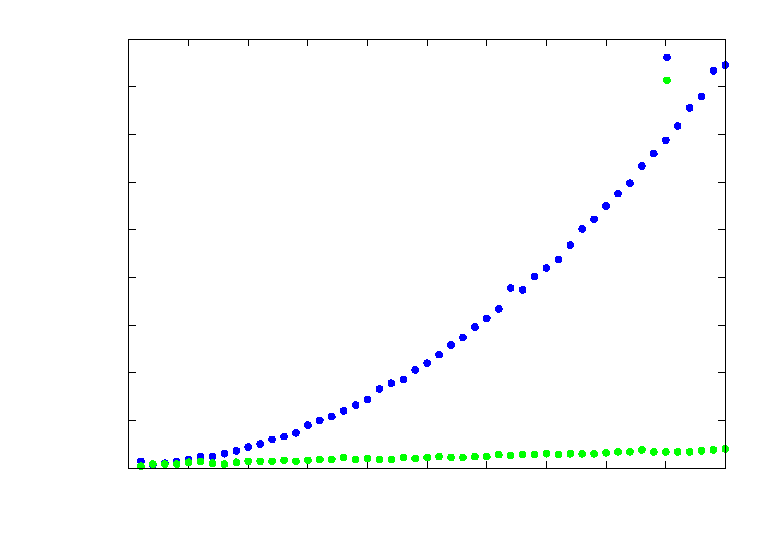
\includegraphics[width={361.00bp},height={253.00bp}]{grafik}}%
    \gplfronttext
  \end{picture}%
\endgroup

\end{figure}


\begin{table}[h]
\centering
    \begin{tabular}{c c c}
        Broj tačaka & Vreme naivni (s) & Vreme pametni (s) \\ \toprule
        5000 & 0.126000 & 0.012000 \\ \midrule
        10000 & 0.437000 & 0.018000 \\ \midrule
        15000 & 0.929000 & 0.026000 \\ \midrule
        20000 & 1.670000 & 0.033000 \\ \midrule
        25000 & 2.651000 & 0.040000 \\ \midrule
        30000 & 3.711000 & 0.048000 \\ \midrule
        35000 & 5.079000 & 0.060000 \\ \midrule
        40000 & 6.659000 & 0.071000 \\ \midrule
        45000 & 8.345000 & 0.071000 \\ \midrule
        50000 & 10.267000 & 0.079000 \\ \bottomrule
    \end{tabular}
    \caption{Tabela sa vremenima izvršavanja za različite veličine ulaza.}
\end{table}
\end{document}
